% Created 2024-03-04 Mon 18:56
% Intended LaTeX compiler: pdflatex
\documentclass[11pt]{article}
\usepackage[utf8]{inputenc}
\usepackage[T1]{fontenc}
\usepackage{graphicx}
\usepackage{longtable}
\usepackage{wrapfig}
\usepackage{rotating}
\usepackage[normalem]{ulem}
\usepackage{amsmath}
\usepackage{amssymb}
\usepackage{capt-of}
\usepackage{hyperref}
\usepackage[margin=0.5in]{geometry}
\usepackage{tikz}
\setcounter{secnumdepth}{2}
\date{}
\title{Does Identity Matter?}
\hypersetup{
 pdfauthor={Rudolf Jovero},
 pdftitle={Does Identity Matter?},
 pdfkeywords={},
 pdfsubject={},
 pdfcreator={Emacs 29.1 (Org mode 9.6)}, 
 pdflang={English}}
\begin{document}


\section{Does Personal Identity Matter?}
\label{sec:org1a2301a}
\subsection{History}
\label{sec:orgff30f97}
\subsubsection*{René Descartes and prior}
\label{sec:org6cd0abb}
The self is an immaterial soul, formed of a different substance outside of our physical reality (Dualism).

\subsubsection*{David Hume}
\label{sec:org2e5350b}
David Hume considered the self (or possibly eliminated the self, and instead viewed the self) as a bundle of impressions through time (i.e. original impressions such as perceptions, and secondary impressions such as beliefs, thoughts, and desires).

\subsubsection*{Derek Parfit}
\label{sec:org9da1726}
Derek Parfit builds upon this conception of the self by focusing on this connection of mental states.
Parfit also introduces scenarios where the self runs into branching and merging, and introduces the concepts of \emph{psychological continuity} and \emph{psychological connectedness}.

\subsection{Motivations}
\label{sec:org69dd6c5}
Science fiction has provided us with many cases where the concept of the self is challenged.

\subsubsection*{Sci-Fi}
\label{sec:org57d7100}
\begin{itemize}
\item Teleportation accidents (\emph{Star Trek}) -
\label{sec:orgefd4355}
deconstruction fails, or reconstruction occurs in multiple instances.

\item Mind duplication technology (\emph{Altered Carbon}, \emph{Black Mirror}) -
\label{sec:orgbefe28e}
minds are saved and duplicated for purposes of replication later.
\end{itemize}

\subsubsection*{In Real Life}
\label{sec:orga8d9bd6}
There have been instances where people survive with only half a brain, or where the corpus callosum was severed to treat epilepsy.
In the latter case it seemed like there were two sets of consciousnesses/mentalities.

\section{Scope}
\label{sec:org5dcd830}
\subsection{Self resides in the mind}
\label{sec:org568a6d0}
While other theories of the self emphasize the body or the soul,
for the purpose of this discussion,
we will assume the self is contained in our mental properties.
This does assume a functionalist understanding of mental properties.
While genetic and neural dispositions can instantiate a self, in terms of changes to the self, we will assume that the self need not be continued on the same physical hardware it originated from.

\subsubsection*{1000 dollars or 1000 volts}
\label{sec:org73dcd44}
Your brain will get swapped into another body, and the other body's brain will get swapped into yours.
You get to choose whether the other body with your original brain or your original body with the other brain gets 1000 dollars, the other one gets 1000 volts.
Which one would you choose?

\subsection{Personal Identity over time}
\label{sec:org2c6b9f6}
We are specifically discussing identity over time, not identity in an instance.
Concepts such as nationality, sexuality, and sex and gender can be considered impressions/psychological connections in an instant, and we'll treat them all as some of the aspects of the self that can vary over time.
We're more concerned with how the self changes over time.

\subsection{Self vs. identity \(\rho\)}
\label{sec:org21789f6}
\subsubsection*{Survival of the self}
\label{sec:orge7527b4}
We're concerned with whether an entity called the self persists through given scenarios.
Identity \(\rho\) is a specific relation (\(\rho\)) that does not seem to apply in all cases,
yet it seems we would agree that a self persists even if an identity does not.

\subsubsection*{Identity \(\rho\)}
\label{sec:org4b0d125}
Reflexive \[x=x\]
Symmetric \[x=y \rightarrow y=x\]
Transitive \[x=y \wedge y=z \rightarrow x=z\]
The identity \(\rho\) was assumed to be what mattered with the self, before Parfit.
A belief in self that depends on the identity \(\rho\) implies that there is an entity that meets these criteria when a self survives, and no existence of one when a self does not survive.
These properties imply identity as an all-or-nothing, one-to-one relation.
This is the notion of the self that Parfit challenges.

\subsection{Psychological fission}
\label{sec:org091d5ab}
While Parfit does talk about psychological fusion, Methuselah cases, and thought experiments in which all of these conditions occur, I will tentatively limit this discussion to fission cases.
This means we're mainly concerned with the one-to-one aspect of identity.
The case of fission tries to target the one-to-one aspect.
The fusion and Methuselah cases target the all-or-nothing aspect of identity.

\section{Thought Experiment}
\label{sec:org3c894e2}
The main thought experiment we're concerned with are cases of psychological fission.
If we have a mind that divides into multiple instances, can we really say anything about identity?
\\\empty
\\\empty
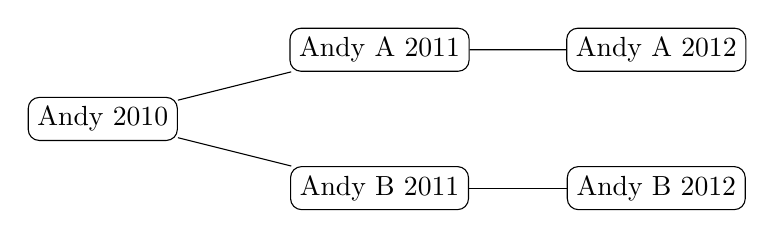
\begin{tikzpicture}
[sibling distance=5em, level distance=10em, grow=right,
every node/.style={shape=rectangle, rounded corners, draw, align=center}]
\node{Andy 2010}
  child{node{Andy B 2011}
    child{node{Andy B 2012}}}
  child{node{Andy A 2011}
    child{node{Andy A 2012}}};
\end{tikzpicture}

\begin{itemize}
\item Andy died in 2011 -
\label{sec:org4b72610}
So a double success is a failure?

\item Either Andy A or Andy B is the only one identical to Andy 2010 -
\label{sec:orge42b6ce}
How do you get to decide who the identical one is?

\item Andy A and Andy B are both Andy 2010 -
\label{sec:org56c1f1a}
If one kills the other, is it both a murder and a suicide?

\item Abandon the assertion of Personal Identity -
\label{sec:orga5dfa88}
The self does not need to be one-to-one. \emph{Psychological continuity} is a better relation to focus on.
\end{itemize}

\section{Implications}
\label{sec:org58a4b99}
\subsection{Law assumes the identity \(\rho\) and it will be a mess if a case of fission occurred.}
\label{sec:org6646224}
\subsection{Self interest's only logical conclusion is generalized altruism.}
\label{sec:org0960d61}
Is it morally right to decide which branch of yourself gets a better life?
\end{document}